\documentclass[oneside,10pt]{book}

\usepackage{cdtBook}
\usepackage{usecases}

\title{Ejercicio 2}
\subtitle{Sistema de Control Escolar, Módulo de Seminarios}
\author{Ingeniería de Software}
%\organization{Escuela Superior de Cómputo, IPN}


%%%%%%%%%%%%%%%%%%%%%%%%%%%%%%%%%%%%%%%%%%%%%%%%%%%%%%%%%%%%%%%%
\begin{document}

\maketitle
\thispagestyle{empty}

\frontmatter
\tableofcontents

\mainmatter

%=========================================================
\chapter{Modelo de Negocios}

\cfinput{reglas}

%=========================================================
\chapter{Modelo de Casos de Uso}
	
	\begin{figure}[htbp!]
		\centering
			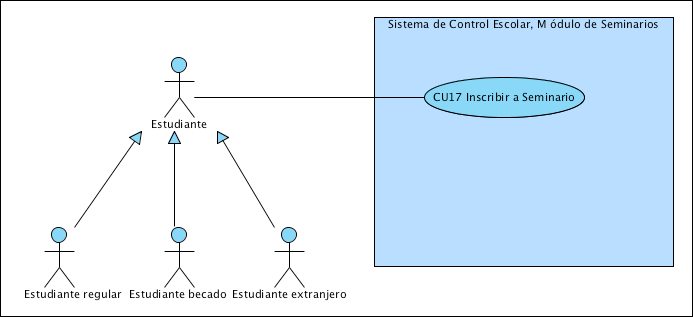
\includegraphics[width=0.8\textwidth]{images/CasosDeUso}
		\caption{Diagrama de Casos de Uso del sistema.}
	\end{figure}
	
\cfinput{cu17/cu}

%%=========================================================
\chapter{Modelo de la Interacción}

{\color{UCInterfaceColor} 
	Esta sección se queda deliberadamente en blanco debido a que el diseño de las interfaces dependerá de la plataforma a utilizar por cada equipo.\\	
}

\cfinput{Pantallas/IU23}


%=========================================================
\chapter{Modelo del Dominio del problema}

	\begin{figure}[htbp!]
		\centering
			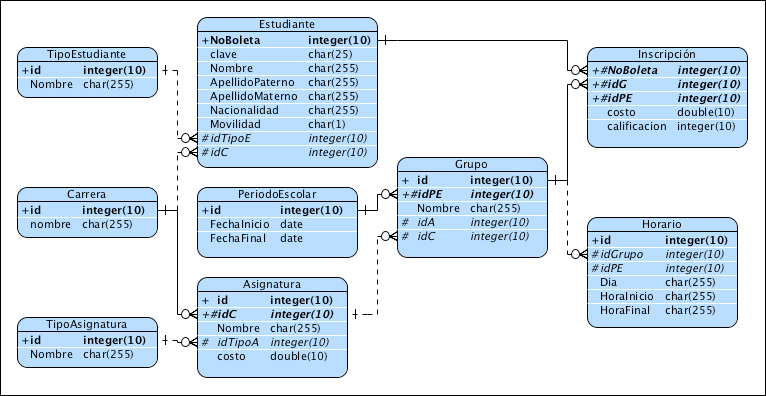
\includegraphics[width=0.8\textwidth]{images/baseDeDatos}
		\caption{Diseño de la Base de Datos.}
	\end{figure}
	
\end{document}
